%TCIDATA{LaTeXparent=0,0,relatorio.tex}



\chapter{Programas utilizados}

\section{Redução modal}
\label {reducaoModalPrograma}
\lstinputlisting[language=Julia]{codes/ModalReduction.jl}

\section{Filtro de Kalman Utilizado, em Linguagem MATLAB --- Adaptado de \cite{GoddardKalmanCode}}
\label {KalmanCode}
\lstinputlisting{codes/KALMAN.m}

\section{Projeto do Controlador com Realimentação de Estados}
\label{projetoControlador}
\lstinputlisting[language=Matlab]{codes/controle.m}

\section{Texto Estruturado}
\label {stsection}

\subsection{Inicialização dos testes}
\label {stMFinit}
\lstinputlisting{codes/initP.st}

\subsection{Inicialização da rede DeviceNET}
\label{dninitST}
\lstinputlisting{codes/InitDNetST.st}

\subsection{Programa de movimentação do motor}
\label{mfprogST}
\lstinputlisting{codes/malhaFechadaP.st}

\newpage

\section{Linguagem \textit{ladder}}
\subsection{Execução de \textit{trigger} da câmera}
\label{laddertrigger}
\begin{figure}[!ht]
\centering
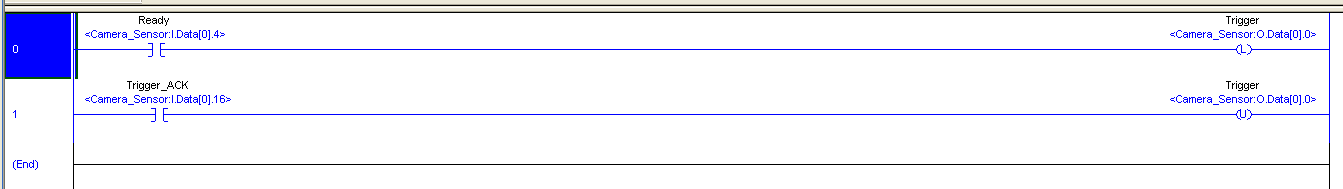
\includegraphics[width=\linewidth]{figs/ladder/camera_trigger}
\caption{\textit{Trigger} da câmera}
\end{figure}

\subsection{Rotina de parada de emergência}
\label{emergencyladder}
\begin{figure}[!ht]
\centering
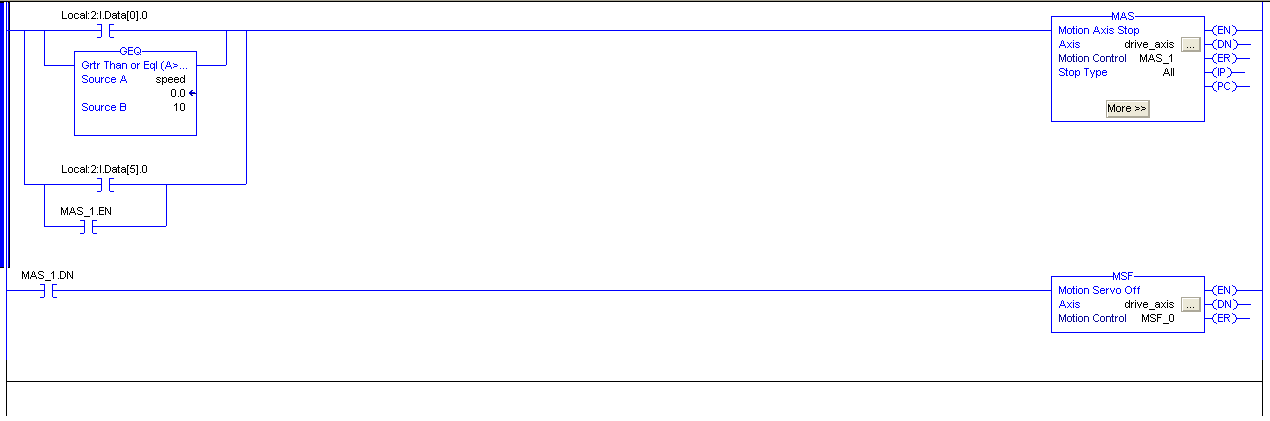
\includegraphics[width=\linewidth]{figs/ladder/emergency}
\caption{Parada de emergência}
\end{figure}

\section{Programas em \textit{Python} para o controle}
\subsection{Exemplo de teste em Malha Aberta}
\label{malhaAbertaAnexo}
\lstinputlisting[language=Python]{codes/testeMalhaAbertaRampa.py}

\subsection{Exemplo de teste em Malha Fechada com Rampa}
\label{malhaFechadaRampaAnexo}
\lstinputlisting[language=Python]{codes/controleSmithPredictorRampa.py}

\subsection{Exemplo de teste em Malha Fechada com Trajetórias Quaisquer}
\label{betterSmithAnexo}
\lstinputlisting[language=Python]{codes/controleSmithPredictor.py}

\newpage

\section{Programas da câmera}
\subsection{Detecção da posição horizontal da bolinha}
\label{ballhorzpos}
\begin{figure}[!ht]
\centering
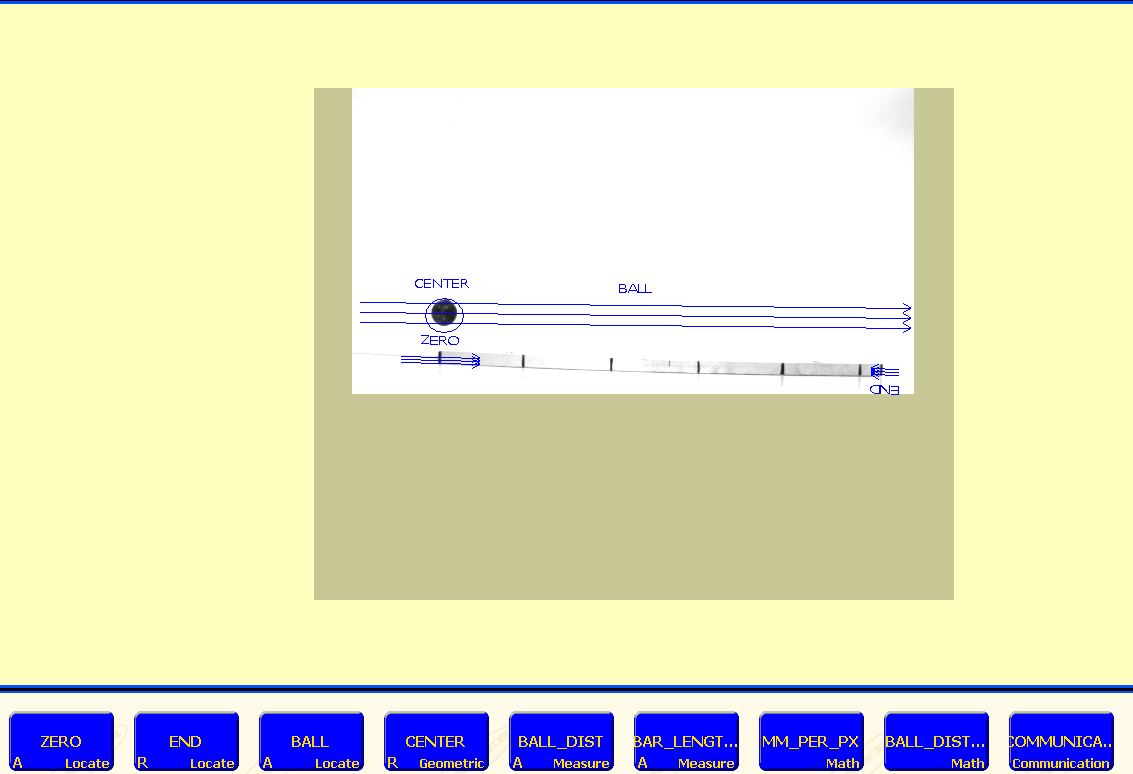
\includegraphics[width=\linewidth]{figs/presence/programaCaptura}
\caption{Detecção da posição horizontal da bolinha}
\end{figure}